\section{Processi organizzativi}

\subsection{Processo di Pianificazione}

Come convenzione il gruppo ha scelto una soglia oraria giornaliera in cui lavorare al progetto. In particolare l'orario di lavoro giornaliero è da considerarsi dalle 9:00 alle 12:00 e dalle 13:00 alle 17:00, per un massimo di 7 ore. Le ore impiegate oltre queste soglie sono considerate ore di \textbf{straordinario}. In particolare al Responsabile è raccomandato pianificare due ore di lavoro al giorno, per un totale di 10 ore settimanali.
		
Il Responsabile, nell'assegnare, task terrà conto di quanto inserito nel calendario, come indicato nel capitolo \ref{Calendario condiviso}, e di quanto indicato nel capitolo \ref{rotazioneruoli} riguardo la rotazione dei ruoli. 

\subsection{Processo di Documentazione}

In questo capitolo vengono descritte le regole adottate per la stesura di tutti i documenti necessari al corretto svolgimento del progetto. Dopo un'attenta valutazione delle varie alternative si è scelto di utilizzare il linguaggio di markup \textbf{\LaTeX{}}. La scelta poggia su diverse motivazioni:

\begin{itemize}

	\item È un linguaggio conosciuto da tutti i membri del gruppo;
	\item Presenta un numero di librerie molto vaste che permettono di realizzare qualsiasi tipo di documento e di personalizzarlo liberamente in modo dettagliato;
	\item La stesura viene fatta su file testuali e non binari, il che agevola il suo versionamento e permette una facile gestione su repository. Inoltre permette di utilizzare facilmente gli script che producono parti di documenti;
	\item È un linguaggio molto diffuso nel mondo informatico e scientifico;
	\item Si può produrre file in formato \glossario{PDF} con estrema facilità grazie al compilatore specifico;
	\item Permette una facile gestione degli indici e dei glossari.
	\item Permette di inserire diagrammi di Gantt, rendendo il loro codice tracciabile e facilmente modificabile.

\end{itemize}

\subsubsection{Template}

Per la stesura dei documenti è stato creato un apposito template \LaTeX{} in cui compaiono tutte le convenzioni sullo stile descritte nel documento corrente. Questo è stato fatto per agevolare il più possibile i componenti del gruppo che andranno a produrre i documenti, in modo che chiunque lavora ad un documento debba preoccuparsi solamente della scrittura del testo senza doversi preoccupare della sua formattazione. 

\subsubsection{Struttura del documento}

	\paragraph{Prima pagina}
	
	La prima pagina del documento deve essere formattata nel modo seguente:
	
	\begin{itemize}
	
		\item \textbf{Logo} del gruppo, visibile come primo elemento centrato orizzontalmente in alto;
		\item Nome del documento, visibile subito dopo il logo, centrato orizzontalmente e marcato come \textbf{titolo};
		\item Una \textbf{tabella} descrittiva, visibile subito dopo il titolo, centrata orizzontalmente e contenente le seguenti informazioni:
			\begin{itemize}
			
				\item \textbf{Versione} del documento, indicata come da norma;
				\item I nomi e cognomi dei \textbf{redattori} del documento;
				\item I nomi e cognomi dei \textbf{verificatori} del documento;
				\item Il nome e cognome del \textbf{responsabile} di progetto, che ha approvato il documento;
				\item Il tipo di \textbf{uso} del documento;
				\item La \textbf{lista di distribuzione} del documento.
			
			\end{itemize}
		\item Una \textbf{descrizione} testuale sommaria del documento, centrata orizzontalmente ed il più possibile sintetica.
	
	\end{itemize}
	
	\paragraph{Registro delle modifiche}
È preferibile che che la numerazione sia continua. La pagina (o le pagine) che seguono devono contenere uno storico di questo documento, in cui verranno riportate tutte le modifiche apportate ad esso. Il registro delle modifiche deve essere composto da una tabella di tante righe quante sono le modifiche apportate ed un numero di colonne pari agli elementi seguenti:
	
	\begin{itemize}
	
		\item Versione del documento;
		\item Data della modifica;
		\item Nome e cognome delle persone coinvolte nella modifica e il ruolo che ricoprono;
		\item Descrizione concisa della modifica apportata.
	
	\end{itemize}
	
	\paragraph{Indice}
	
	Ciascun documento deve contenere un suo indice, in modo da agevolare la consultazione e permettere una lettura \textit{ipertestuale} e non necessariamente sequenziale. Ciascun indice deve essere numerato a partire da 1; per ciascuna sottosezione deve esserci un punto di separazione dalla sezione padre e la numerazione deve di volta in volta ripartire. Per quanto riguarda le appendici esse non devono essere numerate ma indicate da una lettera maiuscola che di appendice in appendice verrà incrementata a partire dalla lettera A seguendo l'ordine alfabetico internazionale.
	
	\paragraph{Formattazione generale delle pagine}
	
	Ciascuna pagina deve rispettare tutti i margini orizzontali e verticali previsti dal template. Ciascuna pagina, ad eccezione della prima, deve contenere un'\textbf{intestazione} (in alto) ed un \textbf{piè di pagina}. Ciascuna intestazione dovrà essere formattata nel modo seguente:

	\begin{itemize}
	
		\item Logo di intestazione del gruppo disposto a sinistra;
		\item Nome del gruppo affiancato al logo;
		\item Titolo del progetto corrente assegnato subito sotto il nome del gruppo;
		\item Numero e titolo della sezione corrente del documento disposto a destra dell'intestazione.
	
	\end{itemize}
	
	Il piè di pagina sarà strutturato invece nel seguente modo:
	
	\begin{itemize}
	
		\item Nome e versione del documento corrente, disposto a sinistra;
		\item Numerazione progressiva della pagina rispetto al totale disposta a destra.
	
	\end{itemize}
	
	\paragraph{Note a piè di pagina}
	
	Per ciascuna pagina interna se dovessero comparire delle note da esplicare esse vanno indicate in basso a sinistra della pagina corrente, riportate con il loro numero e la loro descrizione.

\subsubsection{Versionamento}

Ciascun documento deve essere versionato, in modo che chiunque lo utilizzi possa avere una visione specifica della sua storia e delle sue modifiche. Ad ogni versione deve corrispondere una riga nel registro delle modifiche.

Verrà adottata una numerazione della forma
\begin{center}
 \textbf{v\{X\}.\{Y\}.\{Z\}}
\end{center}

Riguardo a \textbf{\{X\}}:
\begin{itemize}
 \item Parte da 1;
 \item Viene incrementato dal Responsabile di Progetto quando approva il documento;
 \item Quando viene incrementato y e z sono riportati a zero.
 \item Limitato superiormente dal numero di revisioni.
\end{itemize}

Riguardo a \textbf{\{Y\}}:
\begin{itemize}
 \item Parte da 0;
 \item Viene incrementato dal verificatore del documento ad ogni verifica;
 \item Quando viene incrementato z è riportato a zero;
 \item Non è limitato superiormente.
\end{itemize}

Riguardo a \textbf{\{Z\}}:
\begin{itemize}
 \item Parte da 0;
 \item Viene incrementato ad ogni modifica dalla persona che modifica il documento;
 \item Non è limitato superiormente.
\end{itemize}


\subsubsection{Procedura per la definizione di macro personalizzate}

\paragraph{Costanti}

Tutte le macro \LaTeX{} utilizzate come costanti devono iniziare con la lettera maiuscola. Se il nome della macro è composto da più parole unite allora ciascuna deve avere l'iniziale maiuscola e il resto delle lettere minuscolo. Per esempio, \code{\textbackslash NomeDellaCostante} è un nome di costante valido.

\begin{itemize}
	\item Le costanti \textbf{utilizzate da due o più documenti} (es. il nome del gruppo) devono essere definite all'inizio del file \file{root/modello/global.tex};
	
	\item Le costanti \textbf{utilizzate da un solo documento} (es. titolo) devono essere definite nella cartella del documento, all'inizio del file \file{local.tex};
\end{itemize}
	
\paragraph{Funzioni}

Tutte le macro \LaTeX{} utilizzate come funzioni devono iniziare con la lettera minuscola. Se il nome della macro è composto da più parole unite allora ciascuna deve avere l'iniziale maiuscola e il resto delle lettere minuscolo Per esempio, \code{\textbackslash nomeDellaFunzione} è un nome di funzione valido.

\begin{itemize}
	\item Le funzioni \textbf{utilizzate da due o più documenti} (es. il comando che genera la pagina di copertina) devono essere definite nella seconda parte del file \file{root/modello/global.tex};
	
	\item Le funzioni \textbf{utilizzate da un solo documento} devono essere definiti nella cartella del documento che lo utilizza, nella seconda parte di \file{local.tex}.
\end{itemize}

\subsubsection{Norme tipografiche e convenzioni}

Ciascun documento deve rispettare le norme tipografiche definite nella seguente sezione, in modo da rendere il tutto uniforme. Per le situazioni che non sono coperti dalle seguenti norme è preferibile riferirsi a quanto stabilito dall'Accademia della Crusca (\url{http://www.accademiadellacrusca.it}).

	\paragraph{Punteggiatura}
	
	\begin{itemize}

		\item Ciascuna frase deve essere separata da un \textbf{punto} o da un \textbf{punto virgola};
		\item Dopo ogni punto vi dev'essere uno spazio prima dell'inizio della frase successiva;
		\item Ogni frase (ad esclusione di quelle dopo il punto e virgola) deve iniziare con una \textbf{lettera maiuscola};
		\item Per i \textbf{punti di domanda} e i \textbf{punti esclamativi} valgono le stesse regole per i punti;
		\item Dopo ogni \textbf{virgola} deve esserci uno spazio che separa la parte restante della frase;
		\item Dopo ogni \textbf{apostrofo} non deve esserci un carattere di spaziatura;
		\item Ogni elemento di un elenco puntato deve terminare con un punto e virgola, ad eccezione dell'ultimo che deve terminare con un punto;
		\item Ogni elemento di un elenco puntato deve iniziare con una lettera maiuscola.
	
	\end{itemize}
	
	\paragraph{Stile del testo}
	
	Ogni parola di \textbf{glossario} deve essere marcata con una \textit{G} maiuscola a pedice:
	\begin{center}
		\glossario{repository}
	\end{center}

	Ciascuna parola chiave deve essere evidenziata in grassetto. Il \textbf{corsivo} dev'essere utilizzato nei seguenti casi:
	\begin{itemize}
	
		\item \textbf{Citazioni};
		\item \textbf{Abbreviazioni};
		\item \textbf{Riferimenti} ad altri documenti;
		\item \textbf{Parole particolari} solitamente poco usate o conosciute;
		\item \textbf{Nomi di società o aziende};
		\item \textbf{Nome di programmi o \glossario{framework}};
		\item \textbf{Ruoli di progetto};
		\item \textbf{Nome del progetto};
		\item \textbf{Nome del gruppo}.
	\end{itemize}		
	
	\paragraph{Elenchi puntati}
	
	È raccomandato che ciascun elenco puntato sia graficamente rappresentato da un \textit{pallino} nella gerarchia principale e da un trattino nella gerarchia secondaria. Ogni elenco puntato corrisponde ad un concetto che va espresso in modo sintetico. È normalmente preferibile usare elenchi puntati piuttosto che frasi lunghe e discorsive.
	
	\paragraph{Formati}
	
	\begin{itemize}
	
		\item Quando ci si riferisce a una \textbf{data}, se non diversamente specificato, bisogna applicare il formato descritto dallo standard ISO 8601:
		\begin{center}

			\textit{AAAA-MM-GG}
		
		\end{center}
		dove:
		\begin{itemize}

			\item \textit{AAAA} si riferisce all'anno utilizzando quattro cifre;			
			\item \textit{MM} si riferisce al mese utilizzando due cifre;
			\item \textit{GG} si riferisce al giorno utilizzando due cifre.
		
		\end{itemize}
		
		\item Per indicare un \textbf{orario} si usa il formato ventiquattrore nel modo seguente:
		
		\begin{center}

			\textit{hh:mm}		
		
		\end{center}
		dove:
		\begin{itemize}
		
			\item \textit{hh} si riferisce all'ora e può assumere valori da 0 a 23;
			\item \textit{mm} si riferisce al minuto e può assumere valori da 0 a 59.		
		
		\end{itemize}
	
		\item Ogni \textbf{nome} di un membro del gruppo va indicato con il \textit{Nome} seguito dal \textit{Cognome}, a meno che il contesto non richieda diversamente (es. un elenco ordinato per cognome);
		\item Quando ci si riferisce a \textbf{nomi dei file} si deve usare il carattere \texttt{monospace}.
		
	\end{itemize}		
	
	\paragraph{Sigle}
	
	Vengono previste le seguenti sigle:
	
	\begin{itemize}

		\item \textbf{AR} = Analisi dei requisiti;
		\item \textbf{PP} = Piano di progetto;
		\item \textbf{NP} = Norme di progetto;
		\item \textbf{SF} = Studio di fattibilità;
		\item \textbf{PQ} = Piano di qualifica;
		\item \textbf{ST} = Specifica tecnica;
		\item \textbf{MU} = Manuale utente;
		\item \textbf{DP} = Definizione di prodotto;
		\item \textbf{RR} = Revisione dei requisiti;
		\item \textbf{RP} = Revisione di progettazione;
		\item \textbf{RQ} = Revisione di qualifica;
		\item \textbf{RA} = Revisione di accettazione.
	
	\end{itemize}
	
	\paragraph{Riferimenti a documenti}
	
	Quando è necessario riferirsi ai contenuti di un altro documento bisogna specificarne il nome completo e la versione.
	
\subsubsection{Tabelle e immagini}

	\paragraph{Tabelle}
	
	Ciascuna tabella deve essere allineata al centro orizzontalmente e deve contenere sotto di essa la propria didascalia, per agevolarne il tracciamento. In questa didascalia deve comparire il numero della tabella, che dev'essere incrementale in tutto il documento, e una breve descrizione del suo contenuto.
	
	\paragraph{Immagini}
	
	Ogni immagine deve essere centrata orizzontalmente ed avere una larghezza fissa. Inoltre deve essere nettamente separata dai paragrafi che la seguono e la precedono, in modo da definire un netto stacco tra testo e grafica e migliorare conseguentemente la leggibilità. Essa dev'essere accompagnata da una didascalia analoga a quella descritta per le tabelle. Tutti i diagrammi UML vengono inseriti nel documento sotto forma di immagine.
	
\subsubsection{Classificazione di documento}
%	\subsubsection{Bozze}

	\paragraph{Documenti preliminari}
	
	Tutti i documenti sono da ritenersi preliminari fino all'approvazione da parte del Responsabile di Progetto, ed in quanto tali sono da considerarsi esclusivamente ad uso interno.
	
	\paragraph{Documenti formali}
	
	Un documento viene definito formale quando viene validato dal \textit{Responsabile di Progetto}. Solo i documenti formali possono essere distribuiti all'esterno del gruppo. Per arrivare a tale stato il documento deve aver già passato \glossario{verifica} e \glossario{validazione}.
	
	\paragraph{Verbali}
	
	\label{verbale}
	Con verbale ci si riferisce ad un documento redatto da un segretario in occasione  di riunioni interne al gruppo e di incontri con i proponenti. Un verbale viene redatto una prima volta e non subisce successive modifiche, pertanto non é previsto versionamento. \\
	Il verbale dovrà essere approvato dal \textit{Responsabile di Progetto}. Ogni verbale dovrà indicare nel seguente ordine e con il formato indicato:	
	
	\begin{itemize}
		\item Luogo: Città (Provincia), Via, Sede;
		\item Data: dd-mm-yyyy;
		\item Ora: hh-mm 24h;
		\item Partecipanti del gruppo.
	\end{itemize}
	
	Nel primo paragrafo "Informazioni Generali" vanno elencate le informazioni sopra descritte e gli argomenti trattati durante l'incontro. Segue nel secondo paragrafo, Domande e risposte, la trascrizione delle domande poste al proponente e le relative risposte.
	
\subsubsection{Verifica e validazione}

La \textbf{\glossario{verifica}} del documento deve essere eseguita manualmente da parte di un \textit{Verificatore}, scelto dal \textit{Responsabile} tra i membri del gruppo secondo il principio di assenza di conflitti d'interesse, ossia colui che viene chiamato a verificare un determinato componente non può aver in alcun modo partecipato alla creazione. Le verifiche automatizzate sui documenti, dove previste, difficilmente sono esaustive e possono tralasciare delle anomalie. Per eseguire la verifica è necessario controllare che il documento rispetti tutte le norme descritte nelle \textit{Norme di Progetto}.

La \textbf{\glossario{validazione}} del documento consiste nel controllare che il documento abbia \textit{il giusto contenuto}, è un compito che va oltre la semplice verifica delle norme. Richiede una conoscenza a priori del contenuto e degli scopi del documento.
	
	\paragraph{Procedura per la verifica}
	La verifica di un documento è composta come minimo dai seguenti passi:
	\begin{enumerate}
		\item \textbf{Controllo ortografico e del periodo:} con un controllo walktrough bisognerà analizzare i periodi ed eventualmente correggerne la forma, oltre a controllare la presenza di errori ortografici con l'aiuto dello script \code{make test} (vedi sezione \ref{makefile});
		\item \textbf{Verifica delle proprietà di glossario:} con l'aiuto dell'apposito script \code{make test-glossary} (vedi sezione \ref{makefile}) ci si deve assicurare che ogni termite marcato come glossario sia effettivamente definito nel glossario; 
		% \item \textbf{Calcolo dell'indice Gulpease:} per ogni documento redatto, il \emph{Verificatore} deve calcolare l'indice di leggibilità gulpease. Qualora tale indice risultasse troppo basso andranno eseguite le opportune operazioni per semplificare frasi troppo lunghe o complesse;
		\item \textbf{Riportare gli errori frequenti:} per migliorare ciclicamente il processo di verifica, verranno riportati gli errori frequenti. In questo modo sarà più facile eseguire, negli incrementi successivi, controlli di tipo inspection.
		\item \textbf{Segnalazione delle anomalie riscontrate:} il \emph{Verificatore} deve aprire un ticket secondo le modalità descritte nella sezione \ref{aperturaissue}.
	\end{enumerate}

\subsubsection{Approvazione}

L'\textbf{approvazione} di un documento deve essere eseguita dal \textit{Responsabile di Progetto}. Consiste in un accertamento del percorso di vita del documento e serve a fare in modo che soltanto documenti verificati e validati vengano distribuiti ufficialmente all'esterno del gruppo.

\subsubsection{Glossario}

Il \textit{Glossario} contiene le definizioni di tutte le parole che possono creare ambiguità o essere fraintese. Nei documenti tali parole saranno marcate con una G pedice.

Di pari passo con la stesura dei documenti sarà compito degli autori mantenere aggiornato il \textit{Glossario}, inserendo di volta in volta i termini e le relative definizioni. È preferibile inserire nel glossario perlomeno la voce priva di descrizione, per poterla successivamente completare più facilmente.


\subsection{Processo di Verifica}
	Le \glossario{Software Quality Managment Techinques} adottate dal gruppo sono suddivise in quattro categorie. Di seguito ne vengono date le definizioni. Tuttavia non sempre si tratta di classi nettamente distinte e la loro applicazione molto spesso prevede sovrapposizioni.
	Nella pianificazione si cerca di assegnare alla verifica almeno una fetta pari al 30$\%$ delle ore totali.
	
		\subsubsection{Statiche}

		Consiste nello studiare la documentazione ed il software senza istanze di esecuzione del sorgente. Queste tecniche possono includere attività \emph{people-intensive} o di \emph{analisi} condotte da singoli individui con o senza l'assistenza di \glossario{tools} automatizzati.

			\paragraph{Walkthrough} \mbox{} \\
			
			Si svolge effettuando una lettura a largo spettro. È un'attività onerosa e collaborativa che richiede la cooperazione di più persone, si tratta di una tecnica non efficiente pertanto se ne sconsiglia l'attuazione. Ne è previsto l'utilizzo principalmente durante la prima parte del progetto quando non tutti i membri del gruppo hanno piena padronanza e conoscenza delle \emph{Norme di Progetto} e del \emph{Piano di Qualità}.

			\paragraph{Inspection} \mbox{} \\
			\label{anomaliefrequenti}

			Si tratta di una lettura mirata e strutturata, volta a localizzare l'errore con il minor costo possibile. Richiede una buona padronanza di tutti gli strumenti utilizzati e conoscenza di tutti i documenti di progetto. Solitamente viene effettuata da un singolo individuo. La ricerca mirata si basa sugli errori ricorrenti, gli script da utilizzare sono descritti in \ref{makefile}. Le anomalie individuate vanno segnalate secondo le modalità descritte in \ref{aperturaissue}.
			Le anomalie più frequenti sono:
			\begin{itemize}
				\item Utilizzo di comandi locali \LaTeX{} deprecati, ossia quei comandi che erano stati definiti alla prima creazione del \glossario{repository} ma che poi sono stati ridefiniti;
				\item Utilizzo di caratteri di underscore senza prima anteporre una backslash;
				\item Errori ortografici come rappresentare la \emph{È} con una \emph{e} maiuscola apostrofata;
				\item Inserimento di parole comuni come placeholder, e.g. c{}i{}a{}o, b{}l{}a{}b{}l{}a, a{}s{}d \dots; % le parentesi graffe impediscono che make test-regexp trovi queste occorrenze
				\item Formato delle date errato o non conforme alle \NormeDiProgetto{};
				\item Formato dei nomi errato, le \NormeDiProgetto{} indicano prima il nome e poi il cognome;
				\item Elenchi puntati non conformi alle norme, in particolare i punti spesso non terminano con il punto e virgola.
				

			\end{itemize}
			
			
		\subsubsection{People-intensive}

		Sono attività che coinvolgono almeno due persone impegnate a svolgere compiti anche parzialmente non automatizzabili. Solitamente l'efficienza non è massima in quanto si paga il coordinamento tra le persone. Le risorse necessarie sono checklists e i risultati dei tests e delle altre tecniche di analisi.
	
		\subsubsection{Analitiche}

		Le tecniche analitiche comprendono tutte quelle azioni volte a valutare criticamente un componente del prodotto. Tali tecniche si servono di metodi come l'analisi della complessità, degli algoritmi e del controllo di flusso. L'analisi di complessità è utile per valutare quanto un componente è articolato da progettare, implementare, testare o manutenere. Il controllo di flusso è volto al riconoscimento delle anomalie e può essere usato a supporto di altre attività. Infine, l'analisi degli algoritmi è fondamentale in quei software in cui vi è una componente algoritmica importante e vi è la necessità di assicurare output consistenti e corretti. 
				
		\subsubsection{Dinamiche}

		Le tecniche dinamiche vengono generalmente utilizzate durante lo sviluppo e la manutenzione. Si eseguono dei test ripetibili basati sull'effettiva esecuzione del codice. È quindi opportuno costruire un set di strumenti per riprodurre insiemi di \emph{input} e portare il software in uno stato iniziale, al fine di verificare velocemente che gli output siano quelli attesi. Un file di \glossario{log} permetterà, in base al contenuto, di ricostruire le sequenze di operazioni effettuate. Di seguito vengono elencati i test che si andranno ad effettuare in ordine di granularità.\\
		Il \glossario{proponente}, nel corso del \textit{Verbale} del 2013-12-05, ha indicato che dovrà essere testato almeno il  70\% del codice prodotto.
		
			\paragraph{Test di unità} \mbox{} \\

			Si tratta di testare il funzionamento delle \glossario{unità} tramite l'utilizzo di \glossario{stub}, \glossario{test driver}, e \glossario{logger}. Un'\glossario{unità} consiste nella più piccola quantità di software che è utile verificare singolarmente.
			Questi test dovrebbero procedere quanto più in parallelo, assegnando priorità alle \glossario{unità} che mostrano dei risultati utilizzabili per definire dei \glossario{prototipi}. Il corretto funzionamento di tutte le unità riduce al minimo la presenza di errori di programmazione e permette di integrare queste componenti secondo le specifiche di progetto con la garanzia che esse funzionino.
			 
			\paragraph{Test di integrazione} \mbox{} \\

			Consiste nel test di una parte di due o più \glossario{unità} e ne valuta globalmente i risultati. Le componenti non ancora sviluppate vanno simulate con dei sostituti fittizi.
			
			\paragraph{Test di sistema} \mbox{} \\

			Consiste nella validazione del sistema per accertare la copertura dei requisiti software e il suo collaudo viene supervisionato dal committente per mostrare la conformità del prodotto.
			
			\paragraph{Test di regressione} \mbox{} \\

			Consiste nell'eseguire nuovamente i test riguardanti le componenti software che hanno subito modifiche.	Tale operazione è aiutata dal tracciamento, il quale permette di individuare e ripetere facilmente i test di unità, di integrazione e di sistema che sono stati potenzialmente influenzati dalla modifica.
			
			\paragraph{Test di accettazione} \mbox{} \\

			Si tratta del collaudo del prodotto in presenza del proponente. Al superamento di tale collaudo segue il rilascio ufficiale del prodotto sviluppato.

 
 
 \subsection{Strumenti}			
	\subsubsection{Ambiente e strumenti generali}
		
		\paragraph{Sistema operativo}
		
		Il progetto verrà sviluppato su sistemi \textbf{Linux}, per la facilità con cui è possibile preparare l'ambiente di lavoro adatto allo sviluppo dell'applicazione descritta dal capitolato. In particolare è raccomandato il sistema operativo \textbf{Ubuntu} $\geq 12.04$.
%		\paragraph{Installazione componenti aggiuntivi}
		
		\paragraph{Codifica dei caratteri}
		
		Per assicurarsi la corretta visualizzazione dei caratteri accentati tutti i file testuali presenti nel \glossario{repository} devono essere memorizzati con la codifica \textbf{\glossario{UTF-8}}.
		
		\paragraph{Strumenti per il versionamento}
		\label{github}
		
		Per il versionamento dei documenti e del codice viene usato \textbf{Git $\ge$ v1.7.9.5} (\url{http://git-scm.com/}).
		Si utilizzerà il servizio \textbf{GitHub} per creare e gestire i repository privati utilizzati dal gruppo.
		
		
	\subsubsection{Strumenti per la produzione dei documenti}
	
		\paragraph{Scrittura}
		
		Per la stesura dei documenti verrà utilizzato il linguaggio \LaTeX{} (\url{http://www.latex-project.org}).
		Per la stesura sono raccomandati i seguenti editor:
		\begin{itemize}
		 \item \textbf{TexMaker} $\geq 3.2$ (\url{http://www.xm1math.net/texmaker})
		 \item \textbf{Kile} $\geq 2.1.3$ (\url{http://kile.sourceforge.net})
		\end{itemize}
		
		L'output dei documenti sarà in formato \glossario{PDF} e verrà prodotto attraverso il comando \code{pdflatex} (versione $\geq$ 3.1415926-1.40.10-2.2). Per velocizzare questa operazione è stato predisposto il comando \code{make documents}, il cui utilizzo è descritto nella sezione \ref{makefile}.
		
		\paragraph{Strumenti per il controllo ortografico}
		
		Per aiutare il controllo ortografico verrà utilizzato il software \emph{Aspell} (\url{http://aspell.net}, versione $\geq 0.60.7$) con il dizionario italiano.
		
		Per controllare un file \LaTeX{} con \emph{Aspell} l'utilizzo da terminale è il seguente:
\begin{lstlisting}
aspell --lang it --mode tex --encoding utf-8 --personal root/script/aspell_personal.txt --repl root/script/aspell_replacements.txt check {nome del file da controllare}
\end{lstlisting}
		
		Per comodità è stato predisposto il comando \code{make check}, come descritto nella sezione \ref{makefile}.
		
		Quando Aspell segnala un errore su una parola:
		\begin{itemize}
		 \item Se la parola ha un errore ortografico, correggerla scegliendo una delle parole proposte da Aspell oppure usando il comando \textbf{``rimpiazza''};
		 \item Se la parola è scorretta e deve essere modificata tutta la frase, selezionare il comando \textbf{``abbandona''} e fare la modifica utilizzando una \glossario{IDE};
		 \item Se l'errore segnalato da Aspell è un falso positivo, selezionare il comando \textbf{``aggiungi''}.
		\end{itemize}

		\paragraph{Script di Makefile}
		\label{makefile}

Per agevolare molte operazioni è stato predisposto uno script \glossario{Makefile}. Al momento sono previsti i seguenti comandi:
\begin{itemize}

\item \textbf{\code{make test}} \\
Per ogni file \file{*.tex} contenuto nella cartella e nelle sue sotto-cartelle:
\begin{itemize}
	\item Verifica che i file siano memorizzati con la codifica \glossario{UTF-8};
	\item Verifica con \emph{Aspell} che le parole utilizzate nei documenti siano comprese nel dizionario italiano di \emph{Aspell} o nel dizionario personalizzato \\
	\file{root/script/aspell\_personal.txt}.
\end{itemize}
	
\item \textbf{\code{make documents}} \\
Compila tutti i documenti presenti nelle sotto-cartelle.

\item \textbf{\code{make test-glossary}} \\
Controlla che tutti i termini marcati con il comando \code{\\glossario\{\dots\}} siano definiti da un corrispondente comando \code{\\definizione\{\dots\}}.

\item \textbf{\code{make test-regexp}} \\
Per ogni regola della forma \code{grep\_test \{RegExp\} \{Messaggio\} \{File\}} definita internamente allo script controlla se ci sono occorrenze dell'espressione regolare \code{\{RegExp\}} nei file \code{\{File\}}. Per ciascuna occorrenza visualizza il messaggio \code{\{Messaggio\}} seguito dal nome del file e la linea in cui è stata trovata l'occorrenza. È raccomandato usarlo per la verifica dei documenti.

\item \textbf{\code{make gulpease}} \\
Per ogni documento \glossario{PDF} calcola l'indice di leggibilità \glossario{Gulpease} e lo visualizza. Richiede di avere installato il framework \code{python-nltk} e il programma \code{pdftotext}.

\end{itemize}

È possibile eseguire i primi due comandi dalle cartelle dei documenti e dalle loro cartelle superiori, fino alla cartella principale del repository. I restanti comandi si possono eseguire soltanto dalla cartella principale del repository.

\paragraph{UML}
		
	Per la produzione dei diagrammi \emph{\glossary{UML}} verrà utilizzata la piattaforma \emph{Lucidchart}
	(\url{https://www.lucidchart.com}).
		
	È stato valutato anche il software \emph{Astah Professional} (\url{http://astah.net/editions/professional}), utilizzabile con
	una licenza accademica gratuita, ma è stato preferito Lucidchart per la facilità con cui è possibile collaborare online.\\
		
	Per automatizzare il reperimento delle immagini relative ai diagrammi \glossary{UML} si è creato uno script apposito il quale
	scaricherà nella cartella \code{/AnalisiDeiRequisiti/UML} i diagrammi presenti in Lucidchart. \\
	Per utilizzarlo bisogna installare \glossario{ngrok} $\geq 1.3$ e per la prima esecuzione, eseguire le istruzioni nel file
	\code{download$\_$UML.py} nella cartella \code{/AnalisiDeiRequisiti}. \\ 
	Per le esecuzioni successive basterà utilizzare dal terminale il comando: \code{python download$\_$UML.py}.
	
\paragraph{Script download use case e requisiti}
	In \emph{Requisteak} sono presenti le descrizioni degli use case e i requisiti, per effettuarne il download in formato
	\code{.tex} è stato predisposto uno script che andrà a prendere tali informazioni e creerà i corrispettivi capitoli.\\
	 Dopo essersi posizionati all'interno della cartella \code{/AnalisiDeiRequisiti}, eseguire lo script con il comando da terminale:
	 \code{python download$\_$requisiti.py} \\
	

\paragraph{Script di produzione del Gantt e dei grafici}
		\label{Gantt}
Per agevolare la produzione dinamica del \textit{Piano di progetto} è stato scritto un apposito script che genera automaticamente i diagrammi di \glossario{Gantt} e i grafici relativi alla suddivisione del lavoro e al prospetto economico.
Tale script sfrutta le \glossario{API} messe a disposizione da \glossario{TeamworkPM} che permettono di scaricare tutto ciò che riguarda il progetto aperto sulla piattaforma, includendo \glossario{milestone}, persone, TaskList e ore.
Lo script si preoccupa, attraverso le informazioni prelevate, di :
\begin{itemize}
\item Generare in output le tabelle delle ore per ruolo divise per ogni \glossario{milestone} pianificata in \glossario{TeamworkPM} in un corrispondente file \code{.tex},
\item Generare per ogni \glossario{milestone} pianificata, un file \code{.tex} con il corrispondente diagramma di \glossario{Gantt};
\item Generare i grafici a torta riguardanti le ore per ruolo in ogni \glossario{milestone};
\item Generare i grafici a torta riguardanti i costi per ruolo in ogni \glossario{milestone} e in totale;
\item Generare i grafici a barre relativi a ore per ruolo per componente corrispondenti ad ogni \glossario{milestone} e in totale;
\item Effettuare la verifica, con segnalazione di errore se l'esito è negativo e descrizione di tali segnalazioni in un file \code{.txt}, del rispetto delle norme nella pianificazione : 
	\begin{itemize}
	\item Verifica che non siano presenti per ogni persona dei task sovrapposti;
	\item Controlla i vincoli sulle ore per persona;
	\item Controlla i vincoli sul preventivo;
	\item Verifica che la rotazione dei ruoli sia corretta;
	\item Controlla che le ore di verifica siano maggiori del 30$\%$.
	\end{itemize}
\end{itemize} 
Un esempio di parte di output relativo alla funzionalità di verifica delle norme nella pianificazione è dato dalla figura: 
\begin{figure}[H]
    \centering
    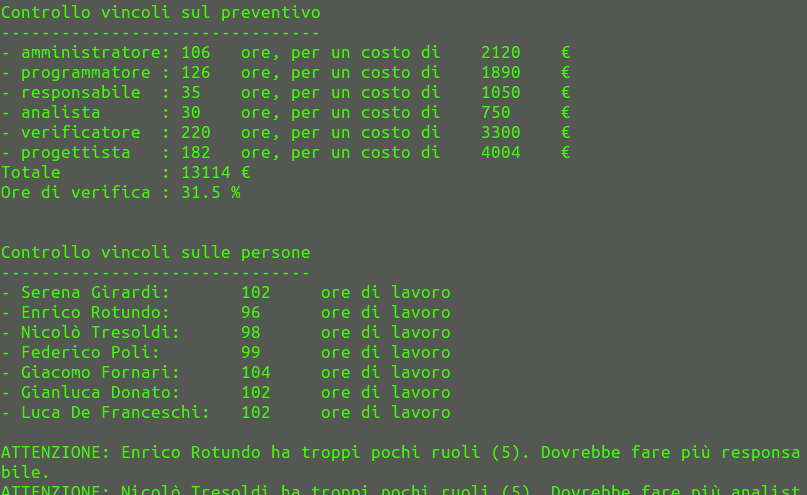
\includegraphics[scale=0.35] {ScriptGantt.png} 
    \caption{Esempio script}
\end{figure}

Per poterlo utilizzare, abilitare le API nel proprio account \glossario{TeamworkPM} per ottenere il token da utilizzare alla richiesta dello script. \\
Eseguirlo da terminale posizionandosi nella cartella \code{/PianoDiProgetto} con il comando \code{python download$\_$gantt.py}.

	\subsubsection{Ambiente e strumenti per la verifica e validazione}

	\paragraph{Strumenti per l'analisi statica}
		Gli strumenti utilizzati per effettuare l'analisi statica del prodotto sono stati
	integrati in uno script \glossario{Makefile}, descritto alla sezione \ref{makefile-codifica}.
		
		Sono stati utilizzati i seguenti software:
		\begin{itemize}
		\item \textbf{JSHint} (\url{http://www.jshint.com}), \glossario{tool} che aiuta a controllare che il codice sorgente rispetti le regole descritte nella sezione \ref{formattazione};
		\item \textbf{Plato} (\url{https://github.com/es-analysis/plato}), \glossario{tool} usato per misurare e visualizzare le metriche descritte nel \PianoDiQualifica{}.
		\end{itemize}
		
		\paragraph{Strumenti per l'analisi dinamica} 
		Gli strumenti utilizzati per effettuare l'analisi dinamica del prodotto sono stati
	integrati in uno script \glossario{Makefile}, descritto alla sezione \ref{makefile-codifica}.
		
		Sono stati utilizzati i seguenti software:
		\begin{itemize}
		\item \textbf{Mocha} (\url{https://github.com/visionmedia/mocha}) Mocha è una libreria ricca di funzionalità per l'esecuzione
		di test Javascript, con esecuzione di quest'ultimi asincrona ed in serie, permettendo segnalazioni flessibili ed accurate.
		\item \textbf{Istanbul} (\url{http://gotwarlost.github.io/istanbul/}) Istanbul è uno strumento che effettua statement, branch, function e line coverage.
		\end{itemize}
		
		\paragraph{Strumenti per la validazione}
		
		Per la validazione delle pagine web si utilizzeranno gli strumenti messi a disposizione da \glossario{W3C} alle pagine 
		 (\url{http://validator.w3.org}) e (\url{ http://jigsaw.w3.org/css-validator}).			
		
		\paragraph{Script di Makefile}
		\label{makefile-codifica}

Per agevolare molte operazioni è stato predisposto uno script \glossario{Makefile} per le attività di codifica. Al momento sono previsti i seguenti comandi:

\begin{itemize}
	\item \textbf{\code{make prepare}} \\
	Prepara l'ambiente di lavoro di Node.js, principalmente scaricando e installando le librerie richieste dal progetto.
		
	\item \textbf{\code{make clean}} \\
	Annulla le operazioni effettuate da \code{make prepare}.

	\item \textbf{\code{make test}} \\
	Esegue i principali script di analisi statica e dinamica. In particolare:
	\begin{itemize}
	\item Controlla la formattazione del codice con JSHint;
	\item Esegue i test d'unità con Mocha.
	\end{itemize}

	\item \textbf{\code{make test-report}} \\
	Esegue gli script di analisi statica e dinamica, inoltre memorizza l'esito in dei file di report interpretabile automaticamente da Jenkins. In particolare:
	\begin{itemize}
	\item Controlla la formattazione del codice con JSHint;
	\item Effettua le misurazioni sul software con Plato;
	\item Esegue i test d'unità con Mocha;
	\item Misura la copertura del software con Istanbul.
	\end{itemize}

	\item \textbf{\code{make jshint}} \\
	Controlla la formattazione del codice con JSHint.
\end{itemize}

È possibile eseguire i comandi soltanto dalla cartella principale del repository del codice.

	\paragraph{Strumenti per l'integrazione continua}
	\label{jenkins}
	
	Grazie all'utilizzo del software \textbf{\glossario{Jenkins}} (v1.548) è stata predisposta un'esecuzione automatica dello script \code{make test-report} ad ogni \glossario{push} effettuato sul \glossario{repository}, in modo da verificare costantemente che le modifiche non introducano errori e che rispettino le metriche software riportate nel \PianoDiQualifica{}.
	
	Ogni build fallita viene notificata all'autore del commit e al Responsabile di progetto via email. Le build che superano la verifica automatica, invece, vengono integrate automaticamente nel branch ``stable'' del repository.
	